\beginsong{Es war ein König in Thule}[wuw={Johann Wolfgang von Goethe, K.F.Zelter, 1812}, bo={140}, pfii={48}, gruen={121}]

\beginverse
\endverse
\centering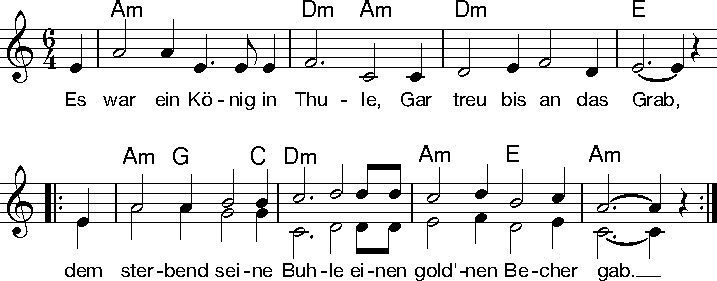
\includegraphics[width=1\textwidth]{Noten/Lied040a.pdf}	

\beginverse
Es \[Am]ging ihm nichts da\[Dm]rü\[Am]ber, er \[Dm]leert' ihn jeden \[E]Schmaus;
\lrep die \[Am]Augen \[G]gingen ihm \[C]ü\[Dm]ber, so \[Am]oft er \[E]trank da\[Am]raus. \rrep
\endverse

\beginverse
Und ^als er kam zu ^ster^ben, zählt' ^er seine Städt' im ^Reich,
\lrep gönnt' ^alles ^seinen ^Er^ben, den ^Becher ^nicht zu^gleich. \rrep
\endverse
 
\beginverse
Er ^saß beim Königs^mah^le, die ^Ritter um ihn ^her,
\lrep auf ^hohem ^Väter^saa^le, dort ^auf dem ^Schloss am ^Meer. \rrep
\endverse

\beginverse
Dort ^stand der alte ^Ze^cher, trank ^letzte Lebens^glut,
\lrep und ^warf den ^heiligen ^Be^cher hi^nunter ^in die ^Flut. \rrep
\endverse

\beginverse
Er ^sah ihn stürzen, ^trin^ken und ^sinken in das ^Meer,
\lrep die ^Augen ^täten ihm ^sin^ken - trank ^nie einen ^Tropfen ^mehr. \rrep
\endverse

\endsong
